\documentclass{article}
\usepackage{tikz}
\usepackage{amsmath}


\begin{document}
\begin{align*}
  & (x, y) - \backslash\mbox{arc}(\theta_1:\theta_2:r) \\ 
  \mbox{center} & = (x-r\cdot \cos(\theta_1), y-r\cdot \sin(\theta_1)) \\
  \mbox{end} & = (x-r\cdot \cos(\theta_1)+r\cdot \cos(\theta_2), y-r\cdot \sin(\theta_1)+r\cdot \sin(\theta_2))
\end{align*}

\begin{center}
  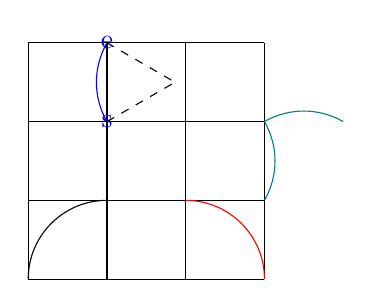
\begin{tikzpicture}
    \draw (0, 0) grid (3, 3);
    \draw (0, 0) arc (180:90:1);  
    \draw[red] (3, 0) arc (0:90:1);  
    \draw[blue] (1, 2)node{s} arc (210:150:1)node{e};  
    \draw[teal] (3, 2) arc (120:60:1);
    \draw[teal] (3, 2) arc (30:-30:1);
    \coordinate (o) at (1.865, 5/2);
    \draw[dashed] (1, 2) -- (o) -- (1, 3); 
  \end{tikzpicture}
\end{center}

three steps to decide $\theta_a,\theta_2$:
\begin{itemize}
  \item Find the center of your circle, Calculate $\Delta x$ between \textbf{start and center}.
  \item Find $\tan\theta_1 = \frac{\Delta y}{\Delta x}$, so that $\theta_1=\theta_0 + \cdots$
  \item Using $\Delta x>0(<0)$ to decide $\cdots$ by $\theta_1\in [-\pi/2, \pi/2]$ or $\theta_1\in [\pi/2,3\pi/2]$
  \item Calculate $\Delta x$ between \textbf{center and end}.
\end{itemize}


\end{document}